\chapter{Methods}
\label{chap-methods}


\section{Disturbance models}

\subsection{Randomly-occurring deterministic disturbances}\label{subsec-RODD}

\textit{Randomly-occurring deterministic disturbances} (RODDs) \citep{macgregor_duality_1984} are a family of stochastic process models suitable for simulating various types of infrequently-occurring disturbances in discrete-time.  The structure of the RODD model is
\begin{equation} \label{eq:RODD}
	p(k)= \frac{B(q^{-1})}{A(q^{-1})}w_p(k),
\end{equation}
where $p(k)$ is the generated disturbance signal, $A(q^{-1})$ and $B(q^{-1})$ are arbitrary polynomial functions of the backward shift operator, $q^{-1}$, and $w_p(k)$ is a random variable generated by a switching system.

To generate randomly-occurring disturbances, the switching system,
\begin{equation} \label{eq:wpk1}
w_p(k) \sim 
\begin{cases*}
	0 & with probability $1-\epsilon$, \\
	\mathcal{N}\left(0, \sigma_{w_p}\right) & with probability $\epsilon$,
\end{cases*}
\end{equation}
may be used, where $w_p(k)$ is either 0 or is sampled from a normal distribution.  When the probability $\epsilon$ is low ($\epsilon<<1$), this system produces \textit{infrequent shocks}.

Alternatively, a mixture of two distributions may be used:
\begin{equation} \label{eq:wpk2}
w_p(k) \sim 
	\begin{cases*}
		\mathcal{N}\left(0, \sigma_{w_p}^2\right) & with probability $1-\epsilon$, \\
		\mathcal{N}\left(0, b^2\sigma_{w_p}^2\right) & with probability $\epsilon$.
	\end{cases*}
\end{equation}

When dealing with a system having more than one RODD, the notation is
\begin{equation} \label{eq:wpik2}
	w_{p,i}(k) \sim 
	\begin{cases*}
		\mathcal{N}\left(0, \sigma_{w_p,i}^2\right) & with probability $1-\epsilon_i$, \\
		\mathcal{N}\left(0, b_i^2\sigma_{w_p,i}^2\right) & with probability $\epsilon_i$.
	\end{cases*},
\end{equation}
where $i \in \left\{1, 2, ..., n_p\right\}$

This approach was taken by \cite{robertson_detection_1995}. In this case, $\sigma_{w_p}$ represents the standard deviation of the noise in periods between random shocks and $b$ is typically large so that the magnitude of the shocks is much greater than the random noise that occurs in the periods between shocks.

Figure \ref{fig:wpk-pdf} illustrates the probability density of $w_p$ in the case of (\ref{eq:wpk2}) with $\sigma_{w_p}=0.01$, $b=100$, and $\epsilon=0.01$. Although it is difficult to discern from the plot, this is a mixture distribution with two components. The component that generates the infrequent shocks is barely visible because of its low probability. In this example, 99 percent of the probability density lies within a narrow range (-0.036 < $w_p(k)$ < 0.036). However, the shocks, which occur with probability 0.01, have much higher amplitude ($b\sigma_{w_p}=1$).

\begin{figure}[htp]
	\centering
	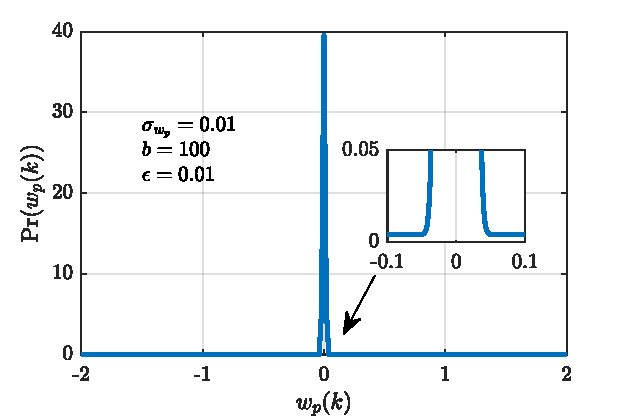
\includegraphics[width=11.5cm]{wpk-pdf-4.pdf}
	\caption{Probability density of a random shock signal}
	\label{fig:wpk-pdf}
\end{figure}

The choice of $A(q^{-1})$ and $B(q^{-1})$ in (\ref{eq:RODD}) determines the nature of the RODD. For example, if $B(q^{-1})=1$ and $A(q^{-1})=1-q^{-1}$, $p(k)$ will be a random-walk process with infrequent, large step changes.

Denoting $\nabla=1-q^{-1}$, the RODD \textit{step-disturbance} process can be defined as
\begin{equation} \label{eq:RODD-step}
	p(k)= \frac{1}{\nabla}w_p(k)
\end{equation}

A RODD \textit{ramp-disturbance} consisting of a series of ramps with randomly-occurring changes in slope may be generated using
\begin{equation} \label{eq:RODD-ramp}
	p(k)= \frac{1}{\nabla^2}w_p(k).
\end{equation}

A RODD consisting of randomly-occurring decaying exponential changes may be generated using
\begin{equation} \label{eq:RODD-exp}
	p(k)= \frac{1}{(1-a_1q^{-1})\nabla}w_p(k),
\end{equation}
where  $0<a_1<1$.

A disturbance with a combination of different RODD types is also possible.  For example, a state-space representation of a RODD combining step changes and ramps is

\begin{equation} \label{eq:RODD-step-ramp}
	\begin{split}
		\mathbf{x}_p(k+1) & =\left[\begin{array}{cc}
			1 & 1 \\
			0 & 1
		\end{array}\right] \mathbf{x}_p(k) +\left[\begin{array}{cc}
			1 & 0 \\
			0 & 1
		\end{array}\right] \mathbf{w}_p(k) \\
		p(k) & =\left[\begin{array}{cc}
			1 & 0
		\end{array}\right] \mathbf{x}_p(k),
	\end{split}
\end{equation}

where $\mathbf{x}_p(k) \in \mathbb{R}^2$ is a state vector and $\mathbf{w}_p(k)$ is a vector of two independent random shock signals generated by (\ref{eq:wpk1}), with possibly different parameter values. Simulated examples of these RODDs are presented in figures \ref{fig:rodd-sim-plots} and \ref{fig:rodd-sim-plot2} in section \ref{chap-simulation}.

\subsection{Hidden Markov Models}

\textit{Hidden Markov models} (HMM) can be used to simulate a more diverse set of switching behaviours than those of the RODD model described in the previous section \citep{wong_realistic_2009}. A Markov process or Markov chain is a stochastic model used to describe a sequence of discrete events in which the probability of future events depends only on the current state. A HMM is a Markov model with states that are not fully observable (i.e. hidden or observed with a measurement error).

To illustrate the basic concept, we can define the state of the random shock generating process (\ref{eq:wpk2}) as a Markov model state $\gamma(k)$ with two possible values:
\begin{equation} \label{eq:gamma-k}
	\gamma(k) = 
	\begin{cases*}
		0: & no shock, \\
		1: & shock.
	\end{cases*}
\end{equation}

$\gamma(k)=0$ represents the state of the process when no shock occurs and $\gamma(k)=1$ represents the state when a shock occurs.

The switching of $\gamma(k)$ can then be defined by a \textit{transition matrix}, $\Pi$, which describes the probabilities of transitioning from the state at time $k$ to the state at time $k+1$:
\begin{equation} \label{eq:Pi}
	\begin{split}
	\Pi = \left(\pi_{ij} \forall i,j\in \{1,2,...,n_j\}\right) \\
	\pi_{ij}=\Pr\left(\gamma(k)=j|\gamma(k-1)=i\right).
	\end{split}
\end{equation}

For example, to simulate the random shock signal used in the RODD model (\ref{eq:wpk2}), the transition probability matrix
\begin{equation} \label{eq:Pi-RODD-step}
	\Pi_{w_{p}} = \begin{bmatrix}
	1-\epsilon & \epsilon \\
	1-\epsilon & \epsilon
	\end{bmatrix}
\end{equation}
is used. In this case, since $w_{p}(k)$ is an independent random variable, it does not depend on the previous state. Therefore, the rows of $\Pi_{w_{p}}$ are identical.

The use of the Markov model thus allows transition probabilities that depend on the current state. For example, consider a disturbance where the signal switches infrequently between samples from two or more distributions with different parameters. The probabilities of switching from one distribution to another may be different. Such a disturbance process could be simulated with a hidden Markov model by conditioning the distribution from which $w_p(k)$ is sampled on the Markov state $\gamma(k)$:
\begin{equation} \label{eq:mog-example}
	\begin{split}
		w_p(k) \sim 
		\begin{cases*}
			\mathcal{N}\left(\mu_{w_p,1}, \sigma_{w_p,1}\right) & if $\gamma(k)=0$, \\
			\mathcal{N}\left(\mu_{w_p,2}, \sigma_{w_p,2}\right) & if $\gamma(k)=1$, \\
			... & ...\\
			\mathcal{N}\left(\mu_{w_p,n_j}, \sigma_{w_p,n_j}\right) & if $\gamma(k)=n_j-1$.
		\end{cases*} \\
	\Pr(\gamma(k)=j|\gamma(k-1)=i)=\pi_{ij} \forall i,j \in {1,2,...,n_j}
	\end{split}
\end{equation}

To make the notation more concise, allow the value of a time-varying discrete variable such as $\sigma_{w_p} \in \left\{\sigma_{w_p,1}, \sigma_{w_p,2},..., \sigma_{w_p,n_j}\right\}$, be determined by the value of the Markov state $\gamma(k)$. Thus,
\begin{equation} \label{eq:A-selection}
	\sigma_{w_p}(\gamma(k)) = 
	\begin{cases*}
		\sigma_{w_p,1} & if $\gamma(k)=0$, \\
		\sigma_{w_p,2} & if $\gamma(k)=1$, \\
		... & ...\\
		\sigma_{w_p,n_j} & if $\gamma(k)=n_j-1$.
	\end{cases*}
\end{equation}


With this notation, (\ref{eq:mog-example}) can be written more concisely as
\begin{equation} \label{eq:mog-example2}
	\begin{split}
		w_p(k) \sim \mathcal{N}\left(\mu_{w_p}(\gamma(k)), \sigma_{w_p}(\gamma(k))\right) \\
		\Pr(\gamma(k)=j|\gamma(k-1)=i)=\pi_{ij} \forall i,j \in {1,2,...,n_j}.
	\end{split}
\end{equation}
where $\mu_{w_p}\in\left\{\mu_{w_p,1},\mu_{w_p,2},...,\mu_{w_p,n_j}\right\}$. This model is known as a \textit{mixture of Gaussians} and can be considered a special-case of a HMM-based disturbance model \citep{wong_disturbance_2007}.

The general HMM disturbance process is described by the following \textit{Markov jump linear system} (MJLS) \citep{costa_discrete-time_2005}. This is a state-space representation with time-varying system matrices $\mathbf{A}(\gamma(k))$, $\mathbf{B}(\gamma(k))$, and $\mathbf{C}(\gamma(k))$:
\begin{equation} \label{eq:HMM}
	\begin{split}
	\mathbf{x}_p(k+1) = \mathbf{A}(\gamma(k))x_p(k) + \mathbf{B}(\gamma(k))\mathbf{w}_p(k) \\
	\mathbf{p}(k) = \mathbf{C}(\gamma(k)) \mathbf{x}_p(k) + \mathbf{e}_p(k)
	\end{split}
\end{equation}

As well as $\mathbf{w}_p(k)$, $\mathbf{e}_p(k)$ may also be a switching random variable. This is a versatile dynamic model suitable for representing and simulating a diverse family of disturbances.

\subsection{Bounded disturbances}

The \textit{bounded random walk} (BRW) is a stochastic process proposed by \citep{nicolau_stationary_2002}. The discrete-time version has the difference equation

\begin{equation} \label{eq:brw}
		p(k+1) = p(k) + a(p(k)) + e(k)
\end{equation}

where $e(k)$ is a random noise with variance $\sigma_e^2$, and $a(p(k))$ is a function defined as

\begin{equation}
	a(x) = e^{\beta}\left(e^{-\alpha_{1}\left(x - \tau\right)} - e^{\alpha_{2}\left(x - \tau\right)}\right)
\end{equation}

where $\beta$, $\alpha_{1}$, and $\alpha_{2}$ are constants.  From (\ref{eq:brw}) it can be deduced that

\begin{equation}
	E(p(k+1)|p(k)) = p(k) + a(p(k)).
\end{equation}

Therefore $a(p(k))$ has the effect of an additive bias or adjustment to $p(k+1)$ which depends on $p(k)$. The shape of $a(x)$ depends on the constants. Figure \ref{fig:brw-a} shows $a(x)$ in the case where $\tau=100$, $\beta=-15$, $\alpha_{1}=3$, and $\alpha_{2}=3$.  From this, it is clear that in the vicinity of $x=\tau$, $a(x)\approx0$. When $a(p(k))=0$, (\ref{eq:brw}) is the equation for a random walk. However, outside a certain neighbourhood around $x=\tau$, $a(x)$ increases for low $x$ or decreases for high $x$. This has the effect of causing $p(k+1)$ to revert towards the mean ($\tau$) whenever $p(k)$ strays outside the neighbourhood. 

\begin{figure}[htp]
	\centering
	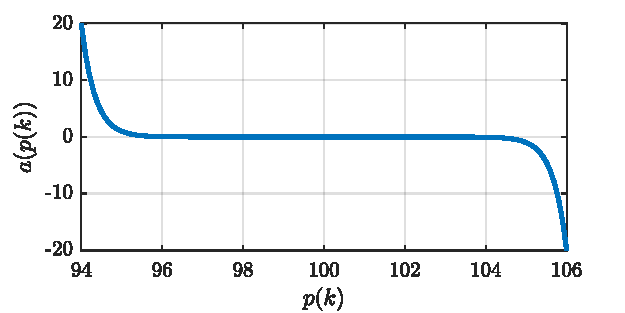
\includegraphics[height=5cm]{images/brw_a.pdf}
	\caption{A bounded random walk bias function}
	\label{fig:brw-a}
\end{figure}

Figure \ref{fig:brw-sim} shows a simulation of a bounded random walk with the parameter values as above, and for comparison, an unbounded random walk (labelled `RW') generated with the same noise input. The dashed lines at $p(k)=95$ and $p(k)=105$ roughly indicate the location of the lower and upper bounds which the BRW only marginally exceeds.

\begin{figure}[htp]
	\centering
	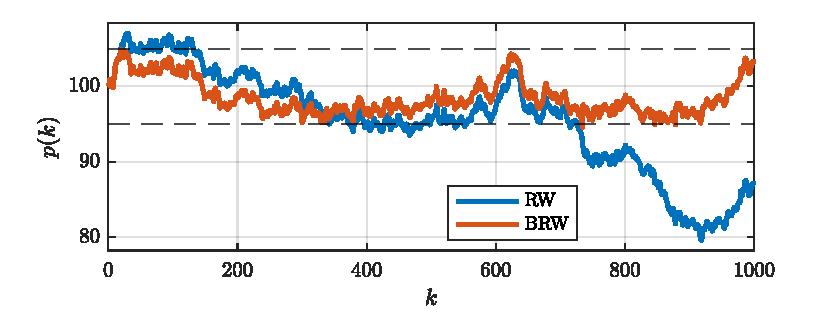
\includegraphics[height=5cm]{images/brw_sim.pdf}
	\caption{Examples of a bounded and unbounded random walk}
	\label{fig:brw-sim}
\end{figure}

Unlike a simple random walk, the BRW is stationary. \cite{nicolau_stationary_2002} derived a formula for the form of the unconditional probability distribution of the continuous-time BRW. Figure \ref{fig:brw-pdf} shows the normalized stationary probability density with the same parameter values as above. For comparison, the probability density of a random walk process after 20 sample periods is also shown. It can be seen that there is a significant probability that the random walk would exceed the bounds of this BRW after 20 sample periods. It can also be seen that the central part of the probability distribution of the BRW is flat, indicating that all values within the bounds are equally likely after a large number of samples, similar to a uniform probability distribution.

%\begin{equation}
%	p_{BRW}(x) \propto \sigma^{-2} \exp \left\{-\frac{2 e^{k}}{\sigma^{2}}\left(\frac{e^{-\alpha_{1}(x-\tau)}}{\alpha_{1}}+\frac{e^{\alpha_{2}(x-\tau)}}{\alpha_{2}}\right)\right\}
%\end{equation}

\begin{figure}[htp]
	\centering
	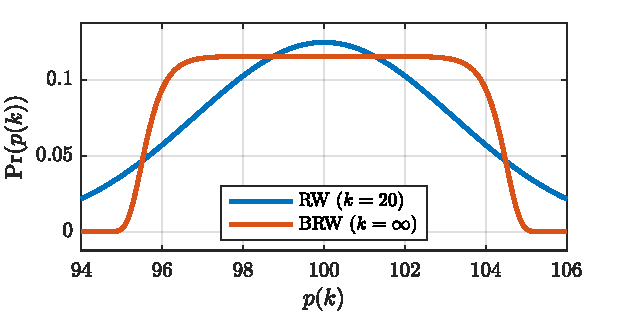
\includegraphics[height=5cm]{images/brw_pdf.pdf}
	\caption{Probability distributions of bounded and unbounded random walks}
	\label{fig:brw-pdf}
\end{figure}

However, the BRW as described by (\ref{eq:brw}) is not guaranteed to be stable.  For extreme values of $p(k)$, $|a(p(k))|$ may be greater than $2|p(k)|$.  This means that $|p(k)|$ will increase rapidly, leading to numerical errors in any practical implementation.  To avoid this, \cite{nicolau_stationary_2002} recommends implementing a regularity condition,
\begin{equation} \label{eq:brw-reg}
	p(k+1) = \tau + \phi(p(k) - \tau) + e(k), \quad \text { if }\left|a(p(k))\right| \geq 2\left|p(k)-\tau\right|,
\end{equation}
where $\phi$ is a constant such that $0<\phi<1$. The size of $\phi$ determines how fast $p(k)$ reverts to $\tau$, the stationary mean of the BRW, when it is outside the stable region.

One drawback of the BRW is that it has a non-Gaussian distribution, making analysis of the properties of any dynamical system with a BRW input difficult.

\section{State estimation}

State estimation is the task of estimating the values of the state variables of a dynamic model of a real system given a set of measurements from the system. In process control applications, state estimates are required online (i.e. in real time), in order to provide the best estimate of the states at the current time, or a prediction of them at the next time instant, based on the available measurements.

Consider the diagram of an input-output system model in Figure \ref{fig:model_diag_uwvy}. Here, $\mathbf{u}(k) \in \mathbb{R}^{n_u}$ is a vector of measured input variables at time instant $k$, $\mathbf{w}(k) \in \mathbb{R}^n$ is a vector of unmeasured state disturbances, $\mathbf{v}(k) \in \mathbb{R}^{n_y}$ is a vector of output disturbances or measurement errors, and $\mathbf{y}(k) \in \mathbb{R}^{n_y}$ is the vector of output variables. The box represents the mathematical model which relates the inputs to the outputs.

\begin{figure}[htp]
	\centering
	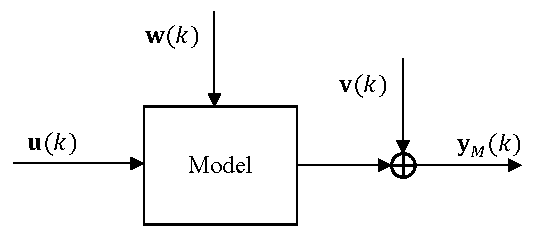
\includegraphics[width=8cm]{images/model_diag_uwvy.pdf}
	\caption{System model diagram}
	\label{fig:model_diag_uwvy}
\end{figure}

The most convenient form in which to represent discrete-time, linear, time-invariant, dynamical system models for state estimation and control purposes, is the state-space representation

\begin{equation} \label{eq:ss_rep_uwy}
	\begin{aligned}
		\mathbf{x}(k+1) = \mathbf{A} \mathbf{x}(k) + \mathbf{B} \mathbf{u}(k) + \mathbf{w}(k), \\
		\mathbf{y}(k) = \mathbf{C} \mathbf{x}(k) + \mathbf{v}(k).
	\end{aligned}
\end{equation}

where $\mathbf{x}(k) \in \mathbb{R}^n$ is a vector of state variables, $\mathbf{A} \in \mathbb{R}^{n \times n}$ is the state transition matrix, $\mathbf{B} \in \mathbb{R}^{n \times n_u}$ is the input matrix, $\mathbf{C} \in \mathbb{R}^{n_y \times n}$ is the output matrix.

\begin{figure}[htp]
	\centering
	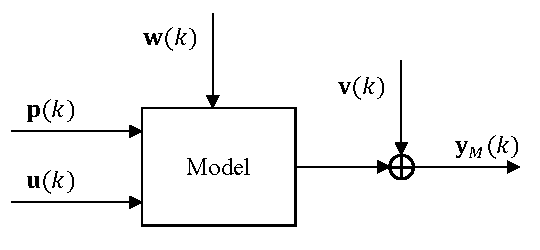
\includegraphics[width=8cm]{images/model_diag_upwvy.pdf}
	\caption{System model with disturbance inputs and manipulatable inputs}
	\label{fig:model_diag_upwvy}
\end{figure}

The \textit{Kalman filter} \citep{kalman_new_1961} is the optimal estimator for a linear system in which the unmeasured disturbances and measurement errors are Gaussian random variables. The predictions of the states at the next time instant, $k+1$, calculated at the current time $k$, are given by
\begin{equation} \label{eq:xkp1_hat}
	\mathbf{\hat{x}}(k+1/k) = \mathbf{A} \mathbf{\hat{x}}(k/k-1) + \mathbf{B}\mathbf{u}(k) + 
	\mathbf{K}(k)\left[\mathbf{y}(k) - \mathbf{C} \mathbf{\hat{x}}(k/k-1)\right],
\end{equation}
where $\mathbf{\hat{x}}(k/k-1)$ is the previous prediction of the states at the current time, calculated in the previous time instant, $\mathbf{y}(k)$ is the current measurement of the output, and $\mathbf{K}(k) \in \mathbb{R}^{n \times n_y}$ is a correction gain matrix. An intuitive interpretation of the Kalman filter is that it iteratively updates the state estimates based on the difference between the output predicted by the system model, $\mathbf{C} \mathbf{\hat{x}}(k/k-1)$, and the output measurement ${y}(k)$.

In the case of a steady-state Kalman filter, $\mathbf{K}(k)$ is constant (time-invariant). However, in general, it is calculated at each time step using
\begin{equation} \label{eq:Kk}
	K(k) = \mathbf{A}\mathbf{P}(k/k-1)\mathbf{C}^\intercal \big(\mathbf{C}\mathbf{P}(k/k-1)\mathbf{C}^\intercal + \mathbf{R}\big)^{-1},
\end{equation}
where $\mathbf{P}(k/k-1)$ is the estimation error covariance matrix calculated in the previous time instant, and $\mathbf{R}$ is the covariance matrix of the measurement noises,
\begin{equation} \label{eq:R}
	\mathbf{R} = E\{ \mathbf{v}(k) \mathbf{v}^\intercal(k) \}.
\end{equation}

$\mathbf{P}(k/k-1)$ is updated every time step using
\begin{multline} \label{eq:Pk}
	\mathbf{P}(k+1/k) = \\ \mathbf{A}\big[\mathbf{P}(k/k-1)
	- \mathbf{P}(k/k-1)\mathbf{C}^\intercal\big(\mathbf{C}\mathbf{P}(k/k-1)\mathbf{C}^\intercal + 
	\mathbf{R}\big)^{-1}\mathbf{C}\mathbf{P}(k/k-1) \big]\mathbf{A}^\intercal + \mathbf{Q},
\end{multline}
where $\mathbf{Q}$ is the covariance matrix of estimation errors,
\begin{equation} \label{eq:Q}
	\mathbf{Q} = E\{ \mathbf{w}(k) \mathbf{w}^\intercal(k) \}.
\end{equation}

The state estimates, $\mathbf{\hat{x}}(k+1/k)$, are calculated recursively online, starting at time $k=0$, using (\ref{eq:xkp1_hat}), (\ref{eq:Kk}) and (\ref{eq:Pk}), provided that initial values of the state estimates, $\mathbf{\hat{x}}(0)$, and estimation error covariance matrix $\mathbf{P}(0)$, are available.

In the case where the system has additional disturbance inputs, $\mathbf{p}(k) \in \mathbb{R}^{n_p}$, as shown in Figure \ref{fig:model_diag_upwvy}, the state-space equations are modified to include these and the input matrix is split into two, $\mathbf{B}_u \in \mathbb{R}^{n \times n_u}$ and $\mathbf{B}_p \in \mathbb{R}^{n \times n_p}$,
\begin{equation} \label{eq:ss_rep_upwy}
	\begin{aligned}
		\mathbf{x}(k+1) = \mathbf{A} \mathbf{x}(k) + \mathbf{B}_u \mathbf{u}(k) + \mathbf{B}_p \mathbf{p}(k) + \mathbf{w}(k), \\
		\mathbf{y}(k) = \mathbf{C} \mathbf{x}(k) + \mathbf{v}(k).
	\end{aligned}
\end{equation}

For state estimation in the presence of disturbances, which is always the case in practice, a suitable model of the disturbances is needed. This additional model is shown in Figure \ref{fig:model_diag_wpupwvy} with an additional set of random variables $\mathbf{w}_p(k)$ at its input.

\begin{figure}[htp]
	\centering
	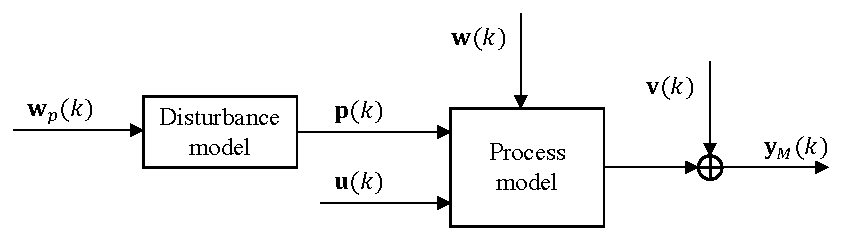
\includegraphics[width=12.5cm]{images/model_diag_wpupwvy.pdf}
	\caption{System with process model and disturbance model}
	\label{fig:model_diag_wpupwvy}
\end{figure}

A state-space representation of the combined system including the disturbance model can be constructed. This will be referred to as the \textit{augmented model},
\begin{equation} \label{eq:ss_rep_xa}
	\begin{aligned}
		\mathbf{x}_a(k+1) = \mathbf{A}_a \mathbf{x}_a(k) + \mathbf{B}_{a,u} \mathbf{u}(k) + \mathbf{B}_{a,w} \mathbf{w}_{a}(k), \\
		\mathbf{y}(k) = \mathbf{C}_a \mathbf{x}_a(k) + \mathbf{v}(k),
	\end{aligned}
\end{equation}
where $\mathbf{x}_a(k) \in \mathbb{R}^{n+n_p}$ is an augmented state vector which includes the states of both the process model and the disturbance model, and $\mathbf{w}_a(k) \in \mathbb{R}^{n+n_p}$ is an augmented vector of random variables (i.e. $\mathbf{w}(k)$ and $\mathbf{w}_p(k)$ combined).


\subsection{Multiple model approaches}

Although the switching of the RODD is unmeasured, it may be observable from the measurements of the outputs of the system. However, as mentioned in Section \ref{chap-lit-review}, systems with RODDs pose problems for state estimation using standard Kalman filters due to the switching of the noise model parameters, namely, the variance of $w_p(k)$ (\ref{eq:wpk2}). As explained by \cite{robertson_detection_1995}, a trade-off must be made during the filter design between its ability to respond to the infrequent disturbance when it occurs, and its sensitivity to noise at other times.

Alternatively, a so-called \textit{multiple-model approach} may be considered \citep{buxbaum_recursive_1970, jaffer_estimation_1971}. Multi-model observers account for different possible hypotheses about the current and past states of the system and infer from these an overall `best' estimate of the current states. To achieve this, an independent Kalman filter is maintained for each hypothesis and a weighted average of the estimates by each filter is calculated using the conditional probabilities of each hypothesis given current and past measurements.

Let the number of Kalman filters be $n_f$ and the \textit{shock occurrence hypothesis} associated with Kalman filter $f$ at time instant $k$ be
\begin{equation} \label{eq:gammak}
	\gamma_{f}(k) \in \left\{0, 1 \right\} \forall{k \ge 0}.
\end{equation}

First, consider the case of estimating only one shock signal (\ref{eq:wpk2}). Therefore, $\gamma_{f}(k)$ is a scalar. The transition probabilities of the random shock are independent of previous shocks:
\begin{equation} \label{eq:Pr_gammak_given_gammakm1}
	\begin{aligned}
		& \Pr\left(\gamma_{f}(k)=0 \mid \gamma_{f}(k-1)\right) = 1-\epsilon, \\
		& \Pr\left(\gamma_{f}(k)=1 \mid \gamma_{f}(k-1)\right) = \epsilon.
	\end{aligned}
\end{equation}

After $k$ time steps, the complete shock occurrence hypothesis associated with filter $f$ is
\begin{equation} \label{eq:Gammak}
	\Gamma_f(k) = \left\{\gamma_f(0), \gamma_f(1), ..., \gamma_f(k) \right\}.
\end{equation}

The measurements up to time $k$ are
\begin{equation} \label{eq:Uk_Yk}
	\begin{aligned}
		\mathbf{U}(k)=\left\{\mathbf{u}(0), \mathbf{u}(1), ..., \mathbf{u}(k) \right\} \\
		\mathbf{Y}(k)=\left\{\mathbf{y}(0), \mathbf{y}(1), ..., \mathbf{y}(k) \right\}.
	\end{aligned}
\end{equation}

Assume that new measurement data is made available at each time instant. The probability of the shock sequence associated with filter $f$ given the data up to time $k-1$ can be calculated recursively:
\begin{multline} \label{eq:Pr_Gammakp1_given_Yk}
	\Pr(\Gamma_f(k) \mid \mathbf{Y}(k-1)) = 
	\Pr(\gamma_f(k) \mid \gamma_f(k-1)) \Pr(\Gamma_f(k-1) \mid \mathbf{Y}(k-1)).
\end{multline}
The conditional probability densities of the measurements $\mathbf{y}(k)$ are approximated by Gaussian distributions
\begin{equation} \label{eq:p_yk_given_Gammak_Ykm1}
	p(\mathbf{y(k)} \mid \Gamma_f(k), \mathbf{Y}(k-1)) \approx
	\mathcal{N}\left(\mathbf{y}(k), \mathbf{C} \mathbf{\hat{x}}_{f}(k/k-1), \mathbf{C} \mathbf{P}_f(k/k-1) \mathbf{C}^\intercal+\mathbf{R}\right)
\end{equation}
where $p(\cdot)$ here represents a probability density function, $\mathbf{\hat{x}}_{f}(k/k-1)$ and $\mathbf{P}_f(k/k-1)$ are the state estimates and estimate covariances of each Kalman filter at the previous timestep, and $\mathcal{N}(\mathbf{y}, \mathbf{\mu}, \Sigma)$ is the multivariate normal probability density of $\mathbf{y}$ with mean $\mathbf{\mu}$ and variance $\Sigma$.

The estimate of the probability of the shock sequence $\Gamma_f(k)$ given the data up to time $k$ is
\begin{equation} \label{eq:Pr_Gammak_given_Yk}
	\Pr(\Gamma_f(k) \mid \mathbf{Y}(k)) = \frac{q_f(k)}{\sum_{f=1}^{n_f} q_f(k)},
\end{equation}
where
\begin{equation} \label{eq:qfk}
	q_f(k) = p(\mathbf{y}(k) \mid \Gamma_f(k), \mathbf{Y}(k-1)) \Pr(\Gamma_f(k) \mid \mathbf{Y}(k-1)).
\end{equation}

The Kalman filters for tracking each hypothesis use the state-space representation of the augmented system model (\ref{eq:ss_rep_xa}). 
However, in the case of a system with a RODD, the disturbance inputs include the non-Gaussian random variable, $\mathbf{w}_p(k)$, as well as the usual Gaussian disturbances on the rest of the states, $\mathbf{w}(k)$:
\begin{equation} \label{eq:wak}
	\mathbf{w}_a(k) = \begin{bmatrix}
		\mathbf{w}(k) \\
		\mathbf{w}_p(k)
	\end{bmatrix}.
\end{equation}

The system is therefore a \textit{hybrid dynamical system} because it has a switching noise covariance matrix. Define the set of possible covariance matrices as
\begin{equation} \label{eq:init_Q_R}
	\mathcal{Q} = \left\{\mathbf{Q}_0, \mathbf{Q}_1\right\},
\end{equation}

and, for convenient notation, let $\mathcal{Q}$ be indexed by the shock indicator variable $\gamma_f(k)$:
\begin{equation} \label{eq:init_Q}
	\mathcal{Q}(\gamma_f(k)) = 
	\begin{cases*}
		\mathbf{Q}_0 & if $\gamma_f(k)=0$, \\
		\mathbf{Q}_1 & if $\gamma_f(k)=1$.
	\end{cases*}
\end{equation}

At the start of simulation, filter $f$ has an initial estimate of the states, $\mathbf{\hat{x}}_f(0)$, and an initial estimate covariance $\mathbf{P}_f(0)$. At each time instant, starting at $k=0$, the filter correction gain is updated as in (\ref{eq:Kk})
\begin{equation} \label{eq:Kf}
	K_f(k) = \mathbf{A}\mathbf{P}_f(k/k-1)\mathbf{C}^\intercal \big(\mathbf{C}\mathbf{P}_f(k/k-1)\mathbf{C}^\intercal + \mathbf{R}\big)^{-1},
\end{equation}

the corrected state estimate at time $k+1$ is calculated as in \ref{eq:xkp1_hat}
\begin{equation} \label{eq:xfkp1_hat}
	\mathbf{\hat{x}}_f(k+1/k) = \mathbf{A} \mathbf{\hat{x}}_f(k/k-1) + \mathbf{B}\mathbf{u}(k) + 
	\mathbf{K}_f(k)\left[\mathbf{y}(k)-\mathbf{C} \mathbf{\hat{x}}_f(k/k-1)\right],
\end{equation}

and the estimation error covariance is updated using
\begin{multline} \label{eq:Pfk}
	\mathbf{P}_f(k+1/k) = \mathbf{A}\big[\mathbf{P}_f(k/k-1)
	- \mathbf{P}_f(k/k-1)\mathbf{C}^\intercal\big(\mathbf{C}\mathbf{P}_f(k/k-1)\mathbf{C}^\intercal \\ + 
	\mathbf{R}\big)^{-1}\mathbf{C}\mathbf{P}_f(k/k-1) \big]\mathbf{A}^\intercal + \mathcal{Q}(\gamma_f(k)). \\
\end{multline}

Note the difference between (\ref{eq:Pfk}) and (\ref{eq:Pk}).  Here, $\mathbf{P}_f(k+1/k)$ is dependent on $\gamma_f(k)$, which determines the noise covariance matrix used in the update, whereas in (\ref{eq:Pk}), $\mathbf{Q}$ is time invariant.

Finally, the multi-model observer estimate of the states in the next time instant is the sum of the $n_f$ Kalman filter estimates weighted by their conditional probabilities:
\begin{equation} \label{eq:x_hat}
	\mathbf{\hat{x}}(k+1/k) = \sum_{f=1}^{n_f} \mathbf{\hat{x}}_f(k+1/k) \Pr(\Gamma_f(k) \mid \mathbf{Y}(k))
\end{equation}

Algorithm \ref{alg:afmm} is the iterative algorithm used to execute these computations.

\begin{algorithm}
	\caption{Multiple model observer calculations}  \label{alg:afmm}
	%\algorithmfootnote{$y_0$ denotes the initial value.}
	\begin{algorithmic}
			\Require $\mathbf{A},\mathbf{B},\mathbf{C},\mathbf{\hat{x}}(0), \mathbf{P}(0), \mathcal{Q}, \mathbf{R}, \epsilon, \mathbf{U}(N), \mathbf{Y}(N)$
			\State $\mathbf{\hat{x}}_1(0) \gets \mathbf{\hat{x}}(0)$  \Comment{Initialize Kalman filters}  % \footnotemark
			\State $\mathbf{P}_1(0) \gets \mathbf{P}(0)$
			\State $\Pr(\Gamma_1(k-1)|\mathbf{Y}(k-1))) \gets 1$
			\For{$f \gets 2, n_f$}
			\State $\mathbf{\hat{x}}_f(0) \gets \mathbf{\hat{x}}(0)$
			\State $\mathbf{P}_f(0) \gets 10^{10}\mathbf{P}(0)$
			\State $\Pr(\Gamma_f(k-1)|\mathbf{Y}(k-1))) \gets 1^{-10}$
			\EndFor
			\For{$k \gets 0, N$}
			\State $\Gamma_f(k), \mathbf{\hat{x}}_f(k), \mathbf{P}_f(k) \gets ...$ \Comment{Sub-optimal procedure occurs here}  % \footnotemark
			\For{$f \gets 1, n_f$}
			\State calculate $\Pr(\Gamma_f(k) \mid \mathbf{Y}(k))$ (\ref{eq:Pr_Gammakp1_given_Yk}, \ref{eq:p_yk_given_Gammak_Ykm1}, \ref{eq:Pr_Gammak_given_Yk}, \ref{eq:qfk})
			\State calculate $\mathbf{K}_f(k)$ (\ref{eq:Kf}) \Comment{Filter updates}
			\State calculate $\mathbf{\hat{x}}_f(k+1/k)$ (\ref{eq:xfkp1_hat})
			\State update $\mathbf{P}_f(k+1/k)$ (\ref{eq:Pfk})
			\EndFor
			\State calculate $\mathbf{\hat{x}}(k+1/k)$ (\ref{eq:x_hat}) \Comment{State estimate}
			\State calculate $\mathbf{P}(k+1/k)$ \Comment{Error covariance}  % \footnotemark
			\EndFor
		\end{algorithmic}
\end{algorithm}

% Version with footnotes - not working
%\begin{algorithm}
%	\caption{Multiple model observer calculations} \label{alg:afmm}
%	%\algorithmfootnote{$y_0$ denotes the initial value.}
%	\begin{algorithmic}
%		\Require $\mathbf{A},\mathbf{B},\mathbf{C},\mathbf{\hat{x}}(0), \mathbf{P}(0), \mathcal{Q}, \mathbf{R}, \epsilon, \mathbf{U}(N), \mathbf{Y}(N)$
%		\State $\mathbf{\hat{x}}_1(0) \gets \mathbf{\hat{x}}(0)$  \Comment{Initialize Kalman filters\footnotemark}
%		\State $\mathbf{P}_1(0) \gets \mathbf{P}(0)$
%		\State $\Pr(\Gamma_1(k-1)|\mathbf{Y}(k-1))) \gets 1$
%		\For{$f \gets 2, n_f$}
%		\State $\mathbf{\hat{x}}_f(0) \gets \mathbf{\hat{x}}(0)$
%		\State $\mathbf{P}_f(0) \gets 10^{10}\mathbf{P}(0)$
%		\State $\Pr(\Gamma_f(k-1)|\mathbf{Y}(k-1))) \gets 1^{-10}$
%		\EndFor
%		\For{$k \gets 0, N$}
%		\State $\Gamma_f(k), \mathbf{\hat{x}}_f(k), \mathbf{P}_f(k) \gets ...$ \Comment{Sub-optimal procedure occurs here\footnotemark}
%		\For{$f \gets 1, n_f$}
%		\State calculate $\Pr(\Gamma_f(k) \mid \mathbf{Y}(k))$ (\ref{eq:Pr_Gammakp1_given_Yk}, \ref{eq:p_yk_given_Gammak_Ykm1}, \ref{eq:Pr_Gammak_given_Yk}, \ref{eq:qfk})
%		\State calculate $\mathbf{K}_f(k)$ (\ref{eq:Kf}) \Comment{Filter updates}
%		\State calculate $\mathbf{\hat{x}}_f(k+1/k)$ (\ref{eq:xfkp1_hat})
%		\State update $\mathbf{P}_f(k+1/k)$ (\ref{eq:Pfk})
%		\EndFor
%		\State calculate $\mathbf{\hat{x}}(k+1/k)$ (\ref{eq:x_hat}) \Comment{State estimate}
%		\State calculate $\mathbf{P}(k+1/k)$ \Comment{Error covariance\footnotemark}
%		\EndFor
%	\end{algorithmic}
%\end{algorithm}
%
%\addtocounter{footnote}{-3} %3=n
%\stepcounter{footnote}\footnotetext{To initialize the bank of $n_f$ Kalman filters, initialize one with an available estimate and covariance of the initial state of the system and set the covariances of all others to high values to ensure they are eliminated as soon as better estimates are available.}
%\stepcounter{footnote}\footnotetext{At this point, the algorithm must extend the shock indicator sequences to the current time instant, while limiting the total number of hypotheses and filters according to a particular sub-optimal method such as the procedures described in section \ref{subsec-pruning} and \ref{subsec-fusion}.
%\stepcounter{footnote}\footnotetext{The estimation error covariance is not required by the algorithm. It may be calculated if needed.}

\subsection{Sub-optimal algorithms}

\begin{itemize}
	\item Sub-optimal algorithms (Tugnait)
	\item Approximation 1: Infrequently-occurring disturbances -> infrequent branching assumptions.
	\item Approximation 2: Infrequently-occurring disturbances -> less combinations of disturbances.
	\item Approximation 3: Filter fusion - 
	\item Recursive Bayesian estimation for non-Gaussian processes
	\item Generalized Pseudo-Bayesian (GPBn) methodology (Bar-Shalom and Li, 1993).
	\item Alternative sub-optimal approach: Sequence pruning (adaptive) methods 
	\item Describe branching and pruning procedure of AFMM.
	\item Explain how the multi-model observer concept can be used for any MJLS (time-varying A, B, C, D, Q, R matrices).
\end{itemize}

\subsubsection{Sequence fusion} \label{subsec-fusion}

Unlike the random shock signal defined by \cite{macgregor_duality_1984}, Robertson and co. use a signal that is sampled from one of two normal distributions, one with a low variance and the other with a much higher variance. This means that the probability density of the shock signal is conditionally Gaussian, whereas the shock signal used by MacGregor and co. has a non-smooth (i.e. degenerate) probability density function.

Robertson and co. propose a combination of three approximation techniques in their RODD state estimator design. Firstly, they assume that the exact timing of the random shock is not important and consider \textit{detection intervals} of more than one sample period during a shock could have occurred. This is based on the observation that when the correction gain of a Kalman filter is increased, it tends to remain large for several sample periods. Secondly, they rely on the fact that the random shocks occur infrequently and thus more than two (or some low number) of shocks are unlikely to occur in the same detection interval. This further reduces the number of filters required, especially in systems subject to multiple independent disturbances. 

The third approximation is referred to as \textit{sequence fusion} or the \textit{generalized pseudo-Bayes algorithm} \citep{jaffer_estimation_1971, buxbaum_recursive_1970, tugnait_detection_1982}. This is based on the assumption that only differences in the recent values of the shock indicator sequence affect the state estimates. Therefore, sequences whose last $f$ terms are the same can be combined. In other words, the length of the unique sequences which must be maintained is limited to the previous $f$ sample periods.

The first is based on the assumption that correctly estimating the exact timing of the random shocks is not important and therefore a filter that assumes a shock occurred within a short period close to the actual occurrence will be adequate. This is based on the observation that when the correction gain of a Kalman filter is increased at time $k$ due to the assumption of a shock occurrence, it tends to remain large for several sample periods thereafter.

The second approximation is based on the assumption that the random shocks occur infrequently and it is quite unlikely that two or more shocks occur within a short time period. This further reduces the number of filters required, especially in systems subject to multiple independent disturbances.

The third approximation is referred to as \textit{filter fusion} or the \textit{generalized pseudo-Bayes algorithm} \cite{jaffer_estimation_1971, buxbaum_recursive_1970, tugnait_detection_1982}. This is based on the assumption that only differences in the recent values of the shock indicator sequence affect the state estimates. Therefore, sequences whose last $f$ terms are the same can be combined. In other words, the length of the unique sequences which must be maintained is limited to the previous $f$ sample periods.

\subsubsection{Sequence pruning} \label{subsec-pruning}

Sequence pruning involves the online deletion of hypotheses (shock sequences in this case) that have a low probability given the current measurements. The deleted sequences are replaced by new sequences to represent the possible branches at the next sample time of only the most likely sequence. For example, for a system with one infrequently-occurring input disturbance, the most likely shock sequence at the next sample time is the shock sequence estimated to be most likely at the current time extended by the addition of a zero to indicate no shock at the next sample time. However, a shock could occur in the next time period. To account for this possibility, a new shock sequence is generated by making a copy of the current most likely sequence and its associated filter and extending it assuming a shock at the next sample time. This new sequence and filter replace the least likely sequence and observer. Thus, the total number of sequences and independent filters that need to be maintained remains constant. Note that in the case of systems with more than one input disturbance, the number of possible branches of the most likely sequence is higher, and therefore a larger number of sequences and filters will be replaced each time step.

There is one restriction to this pruning rule. A sequence created at sample time $k$ cannot be deleted until sample time $k+n_{min}$ where $n_{min}$ is a \textit{minimum life length} parameter. This is necessary because it can take several sample periods before the filter estimates respond to the change and thus the conditional probability of the new sequence is established.

The AFMM algorithm also includes a procedure for online estimation of the measurement noise covariance, using a forgetting factor to control the speed of adaptation of the estimate.\cite{andersson_adaptive_1985}

\section{System identification}

Outline notes:
\begin{itemize}
	\item Explain Isaksson and Eriksson's perspective on standard system identification approach.
	\item Explain distinction between system detection and system identifcation, reference Isaksson and Eriksson's paper on disturbance classification (whether disturbance at input or output of process).
	\item Introduce other approaches—MLE, EM algorithm (Dempster et al., Wong \& Lee)
	\item Methods proposed by Bemporad (Fitting jump models, 2018 and Jump Box-Jenkins, 2020).
	\item Theory and challenges Costa book. Others?
	\item In recent years, numerical methods to overcome the intractability of the probabilistic integral have received a lot of attention.
	\item Sequential Monte-Carlo methods, (incl. particle filering), Stochastic Variational Inference, ... (read Special issue in IEEE control magazine for an overview of these methods)
\end{itemize}

% Note: may remove this if we aren’t using any formal methods.

\section{Control strategies}

Outline notes:
\begin{itemize}
	\item Optimal control—LQR, LQI for demonstration systems (linear, unconstrained).
	\item Here we adopt the certainty equivalence principle — use a standard MPC with a multi-model observer.
\end{itemize}

\section{Grinding simulation model}

Outline notes:
\begin{outline}
	\1 Describe model with references.
	\1 Simplified flow diagram — Figure \ref{fig:sag-diag}
	\1 Population balance model approach - breakage and selection rates.
    \1 Assumptions and limitations: constant breakage rate model, relationships between speed, media, trajectories,  filling level and breakage not captured.
	\1 Grate, transport delays and cyclone model.
	\1 List the main dynamic variables.
	\1 Outline any significant changes made from Edgar's model
	\1 Figure: simulation results showing steady-state characteristics - e.g. power, grind, and throughput vs. fill level and speed.
	\1 Simulation setup - low level controls implemented.
	\2 Feed water ratio control
	\2 Ore feed simulation.
	\1 Figure \ref{fig:coarse_fine_psd_plot}: Particle size distributions of feed, recirculating load and product - this should help explain steady-state characteristics.
	\1 Figure - Step responses of main process variables to changes in ore properties.
	\1 Selection of particle size distribution as the disturbance variable for this work.
\end{outline}



\begin{figure}[htp]
	\centering
	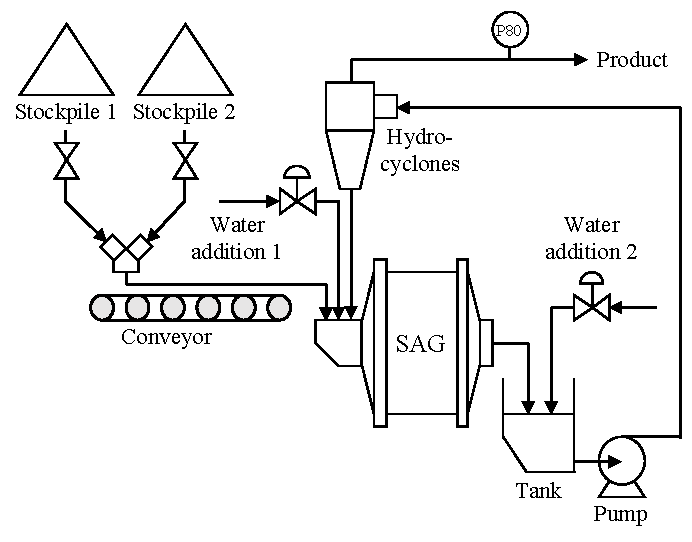
\includegraphics[width=11cm]{images/sag-circuit-diag.pdf}
	\caption{Simplified process flow diagram}
	\label{fig:sag-diag}
\end{figure}

\begin{figure}[htp]
	\centering
	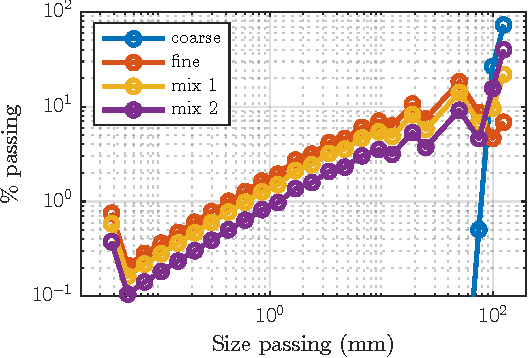
\includegraphics[width=9cm]{images/coarse_fine_psd_plot.pdf}
	\caption{Ore particle size distributions}
	\label{fig:coarse_fine_psd_plot}
\end{figure}

\section{Performance evaluation}

Outline notes:
\begin{itemize}
	\item Comparing disturbance state estimate to true disturbance (simulation only).
	\item Tracking error: Mean-squared difference of output estimates. (or use RMSE?)
	\item Partitioning of simulation outputs into 'transition periods' and steady-state periods.
	\item Variance of output estimate in steady-state (no disturbances).
	\item Mean-squared differences in estimates (similar to variance but with no bias).
	\item Sensitivity to model errors, observer parameters.
	\item Closed loop stability - stability margins.
\end{itemize}

